
\subsection{Best hyperparameters}

Table~\ref{tab:best_configs} summarises the best hyperparameters from the dedicated tuning runs only (\texttt{experiment\_cnn\_tuning} and \texttt{experiment\_lstm\_tuning}). The CNN preferred a large embedding dimension (512), a high number of filters (300), and a learning rate of 0.001. The LSTM preferred a larger hidden dimension (512), embedding dimension 256, bidirectional encoding, and a learning rate of 0.001. Both architectures benefited from very low weight decay (1e-5 or 0.0).


\import{../figures/generated/}{best_config_tuning_only.tex}

\subsection{Test set performance}

Figure~\ref{fig:hyperparameter_devf1_distributions} shows the distribution of dev macro-F1 scores for both models across all hyperparameter search trials. The distributions are relatively tight, especially for the LSTM, indicating that the tuning process was stable and not overly sensitive to hyperparameter choices. The CNN shows a slightly wider distribution, suggesting that its performance may be more sensitive to hyperparameter settings than the LSTM. Overall, both models achieved high dev macro-F1 scores across a range of hyperparameters, which is a positive sign for their generalization capabilities.

\begin{figure}[h]
\centering
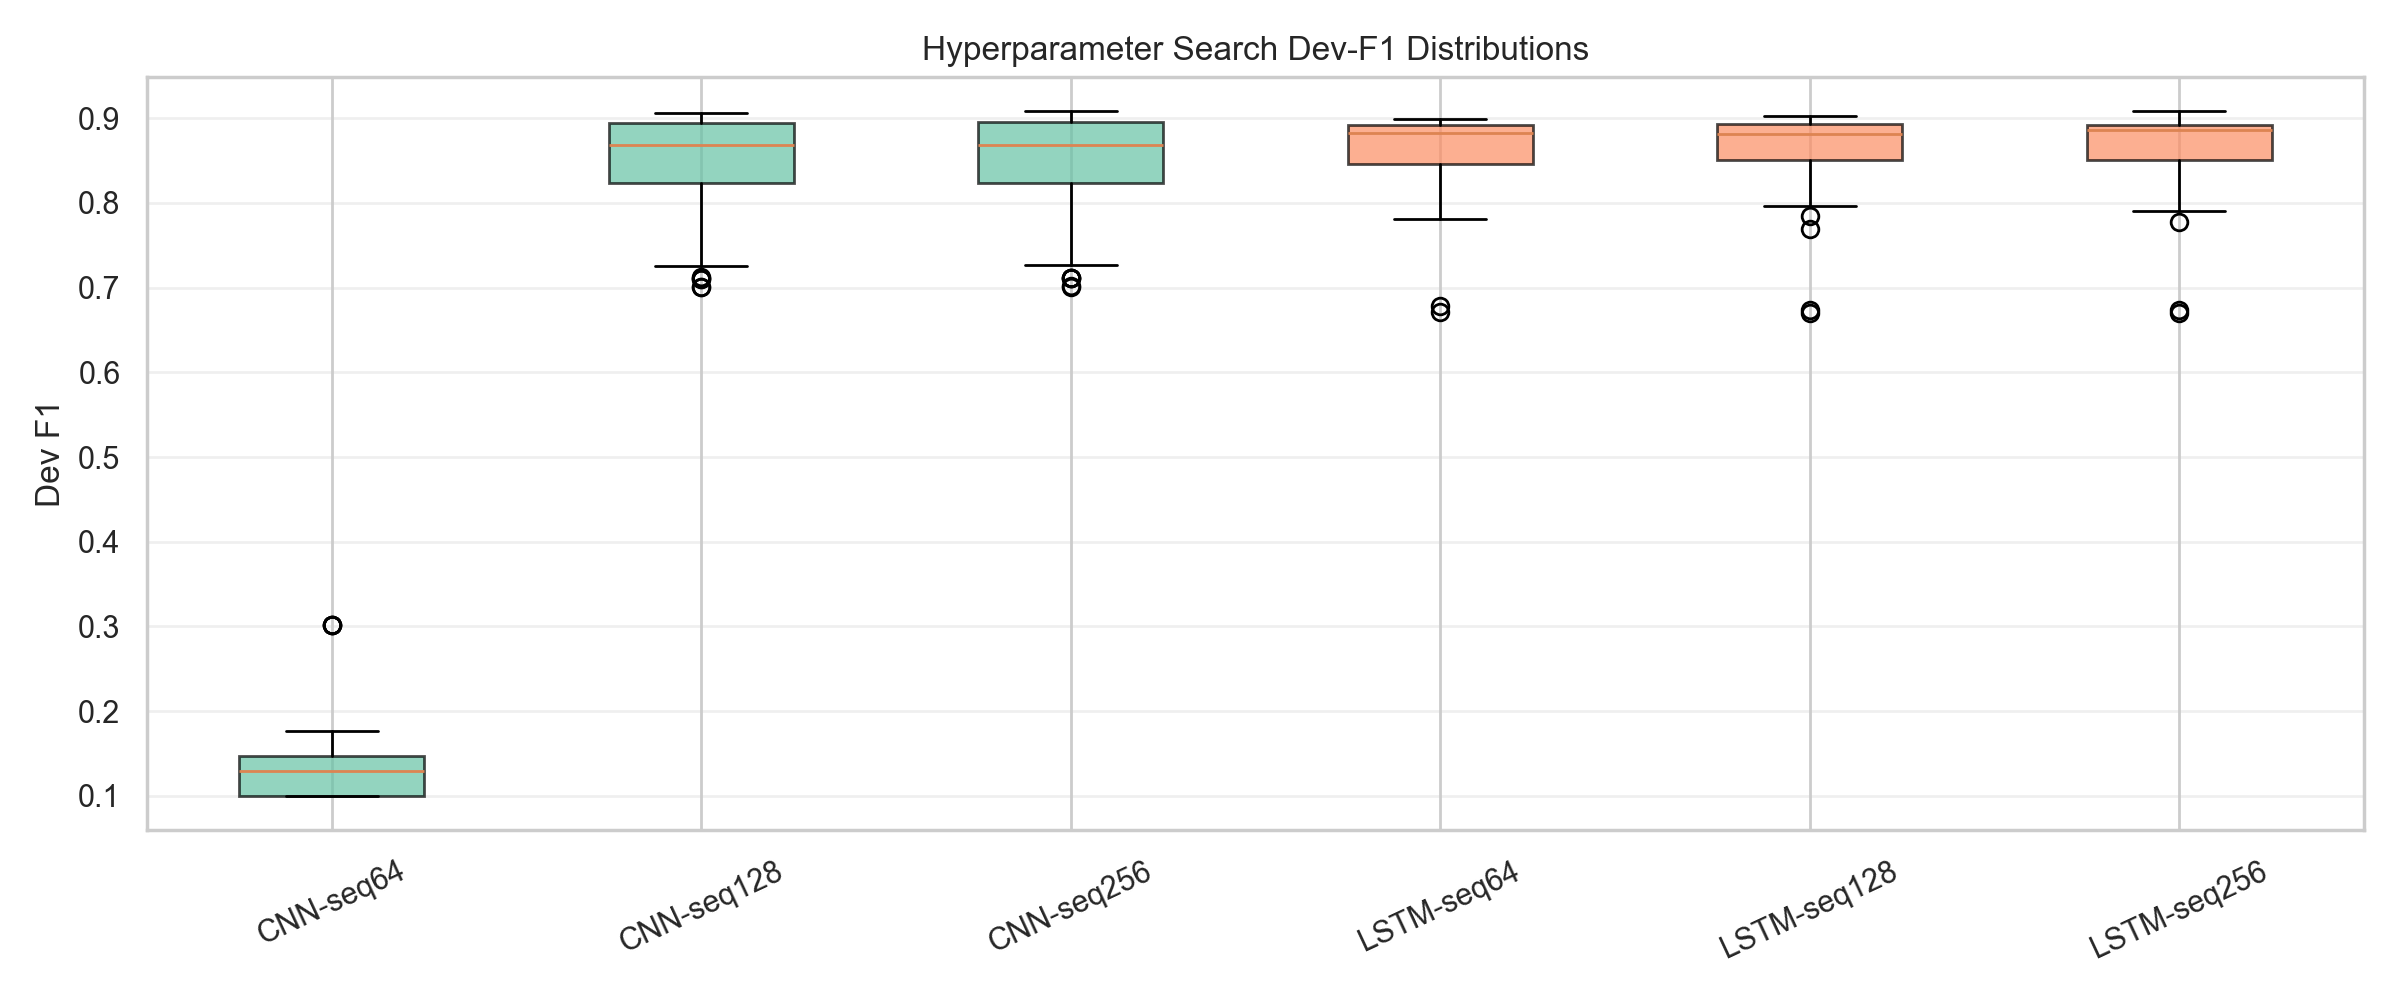
\includegraphics[width=0.5\textwidth]{../figures/generated/hyperparameter_devf1_distributions.png}
\caption{Distribution of dev macro-F1 scores across all hyperparameter search trials, grouped by model. Higher and tighter distributions indicate more stable tuning.}
\label{fig:hyperparameter_devf1_distributions}
\end{figure}


The test results are shown in Table~\ref{tab:test_results}. At the main comparison sequence length of 128 tokens, the CNN slightly outperformed the LSTM, achieving a test accuracy of 90.71\% and a macro-F1 of 90.69\%, compared to the LSTM's accuracy of 90.57\% and macro-F1 of 90.59\%.

Interestingly, the ablation results reveal that longer sequences do not consistently improve performance. For the CNN, the best test macro-F1 was actually achieved at sequence length 64 (90.96\%), while the highest dev F1 was at 256 (91.09\%). The LSTM showed a more monotonic trend, improving from 90.32\% at seq64 to 90.74\% at seq256. The gap between the two models was relatively small across all sequence lengths, with a difference of at most 0.64 percentage points in macro-F1 (at seq64).


\import{../figures/generated/}{test_results_main_vs_ablation.tex}

\subsection{Ablation study: effect of maximum sequence length}

Figure~\ref{fig:test_metrics_vs_seq} shows how test accuracy and macro-F1 vary with sequence length.

\begin{figure}[h]
\centering
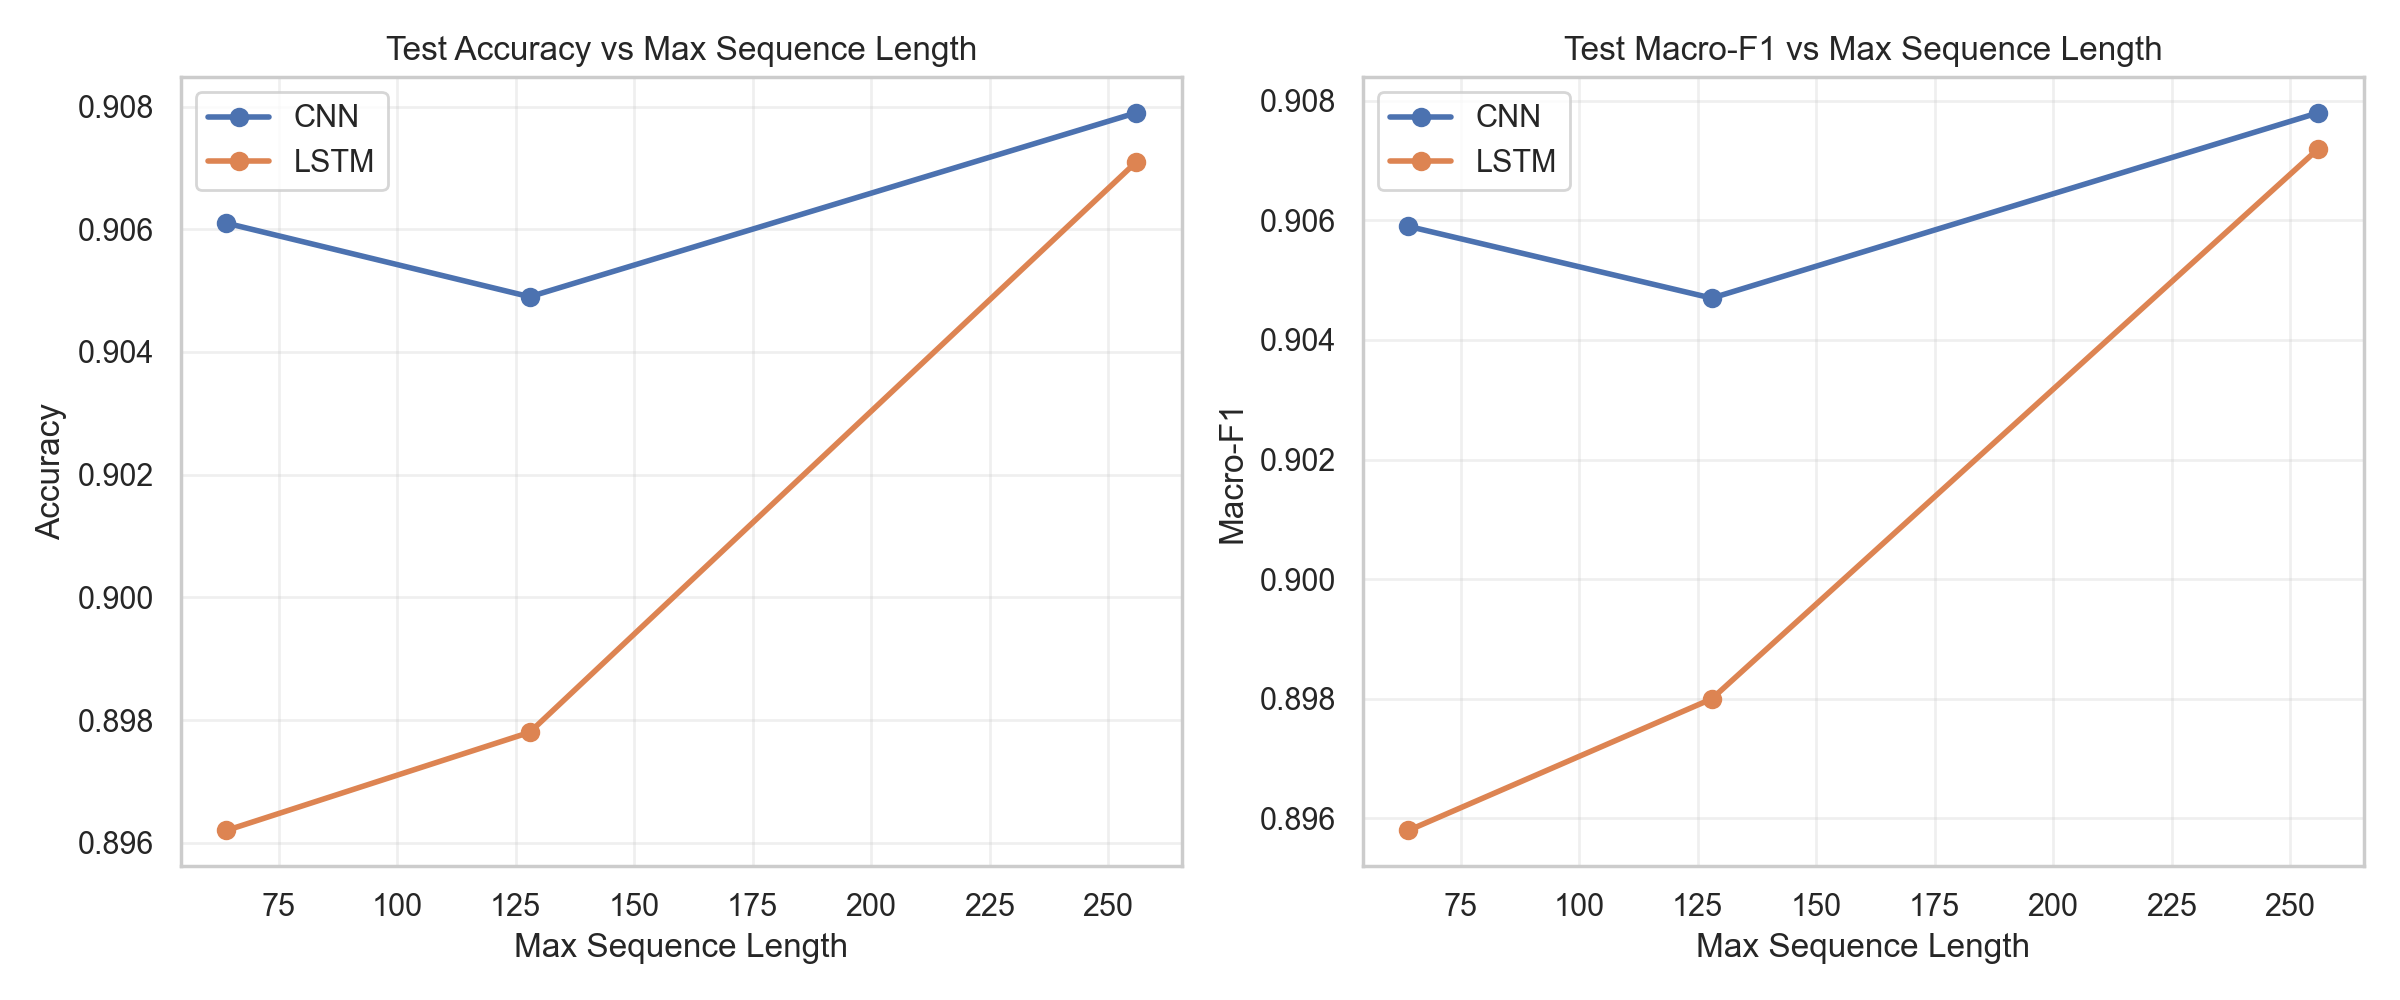
\includegraphics[width=0.95\textwidth]{../figures/generated/test_metrics_vs_seq.png}
\caption{Test accuracy and macro-F1 as a function of maximum sequence length for CNN and LSTM.}
\label{fig:test_metrics_vs_seq}
\end{figure}

The overall trend is clear: The CNN does not benefit from longer sequences, with the best test macro-F1 at seq64. The LSTM, on the other hand, shows a consistent improvement with longer sequences, achieving its best test macro-F1 at seq256. This suggests that the LSTM is better able to leverage the additional context provided by longer input sequences, while the CNN may be more prone to overfitting or may not effectively utilize the extra information. This is especially evident by the fact that the CNN outperforms the LSTM at seq64, but is outperformed by the LSTM at seq256.

\subsection{Class-wise analysis}

Figure~\ref{fig:class_f1_heatmap} presents the per-class macro-F1 scores. The confusion matricies per model and sequence length are shown in Appendix~\ref{app:reports} along with the full classification reports.

\begin{figure}[h]
\centering
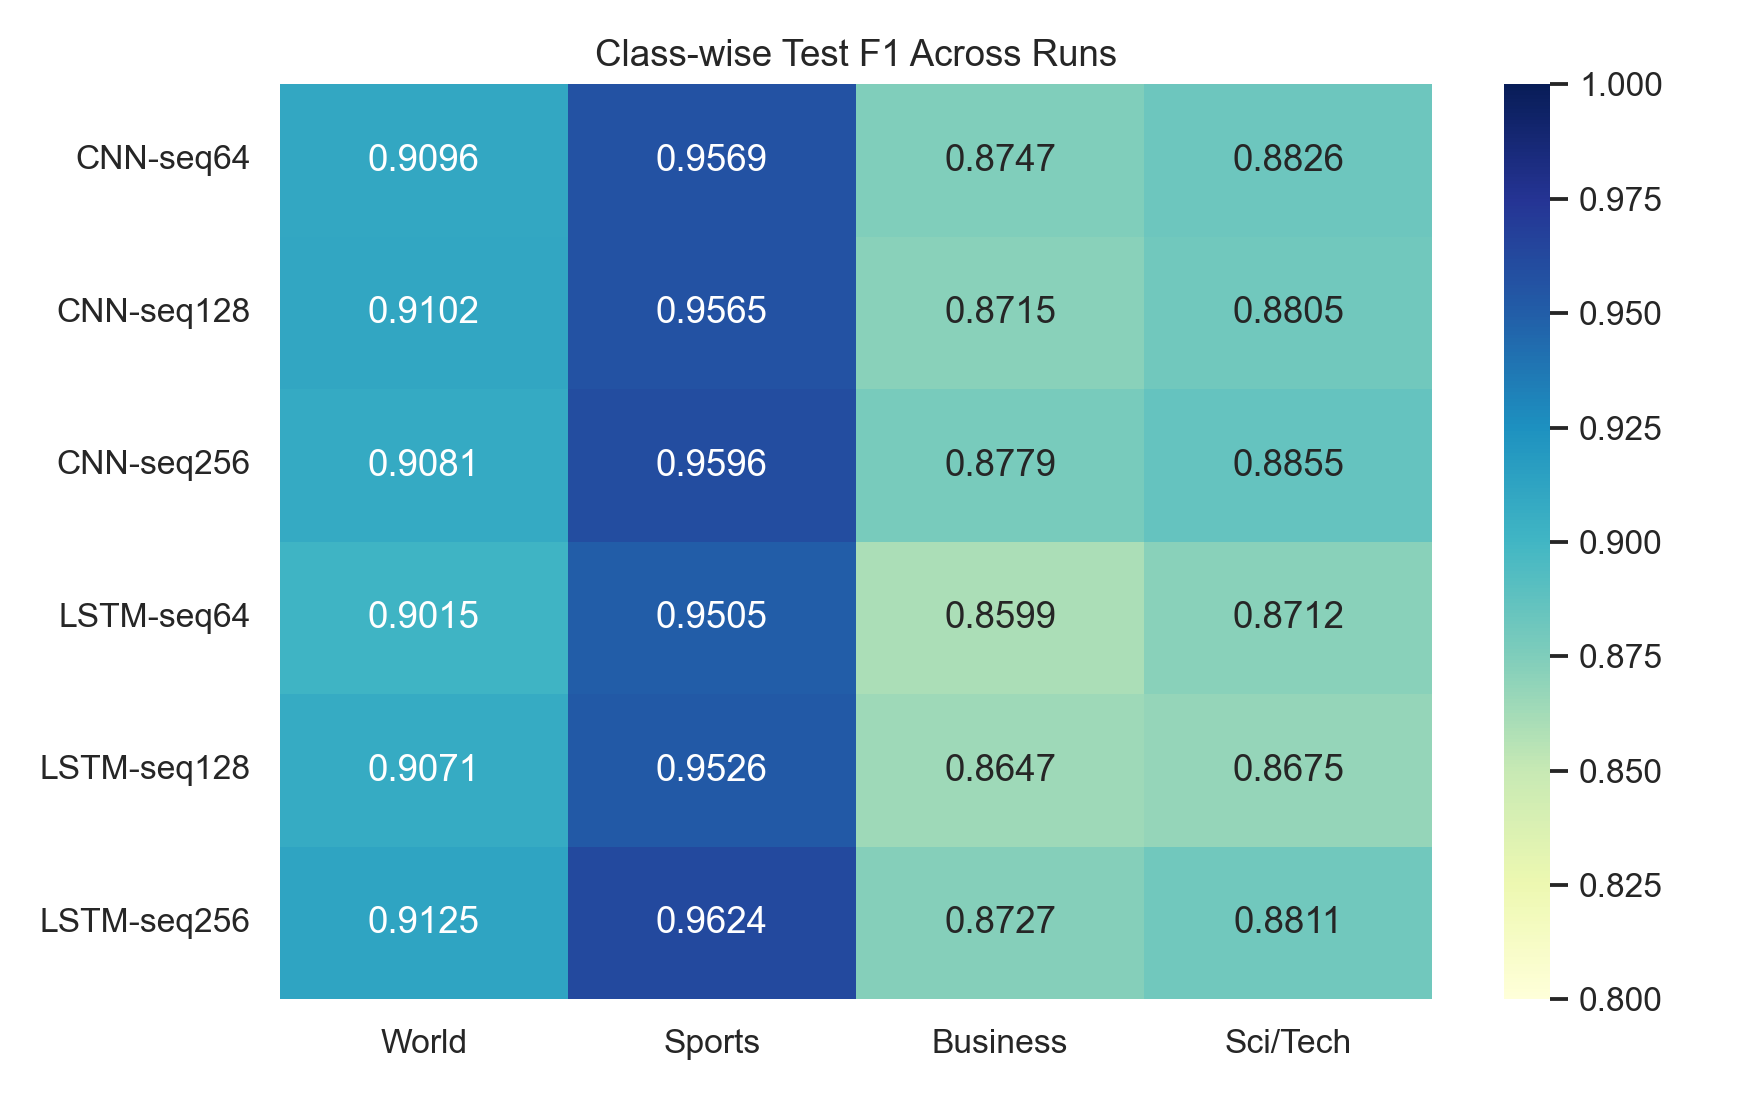
\includegraphics[width=0.85\textwidth]{../figures/generated/class_f1_heatmap.png}
\caption{Heatmap of per-class test F1 scores across all runs. World and Sports are easier to classify; Business is the most challenging.}
\label{fig:class_f1_heatmap}
\end{figure}

The World and Sports classes are generally easier to classify, with F1 scores above 90\% in most configurations. The Sci/Tech class is slightly harder, with F1 scores typically around 87--88\%. The most challenging class is Business, where F1 scores range from 86\% to 87\%, depending on the model and sequence length.


\subsection{Learning curves}

Figure~\ref{fig:full_training_curves_comparison} displays the learning curves for the final training runs on the training set and validation set for all six runs (CNN and LSTM at seq64, seq128, and seq256) with the tuned hyperparameters from the dedicated tuning runs. Both training and validation curves are shown for loss and accuracy. The F1 curves are shown in Appendix~\ref{app:additional_figures}.

\begin{figure}[h]
\centering
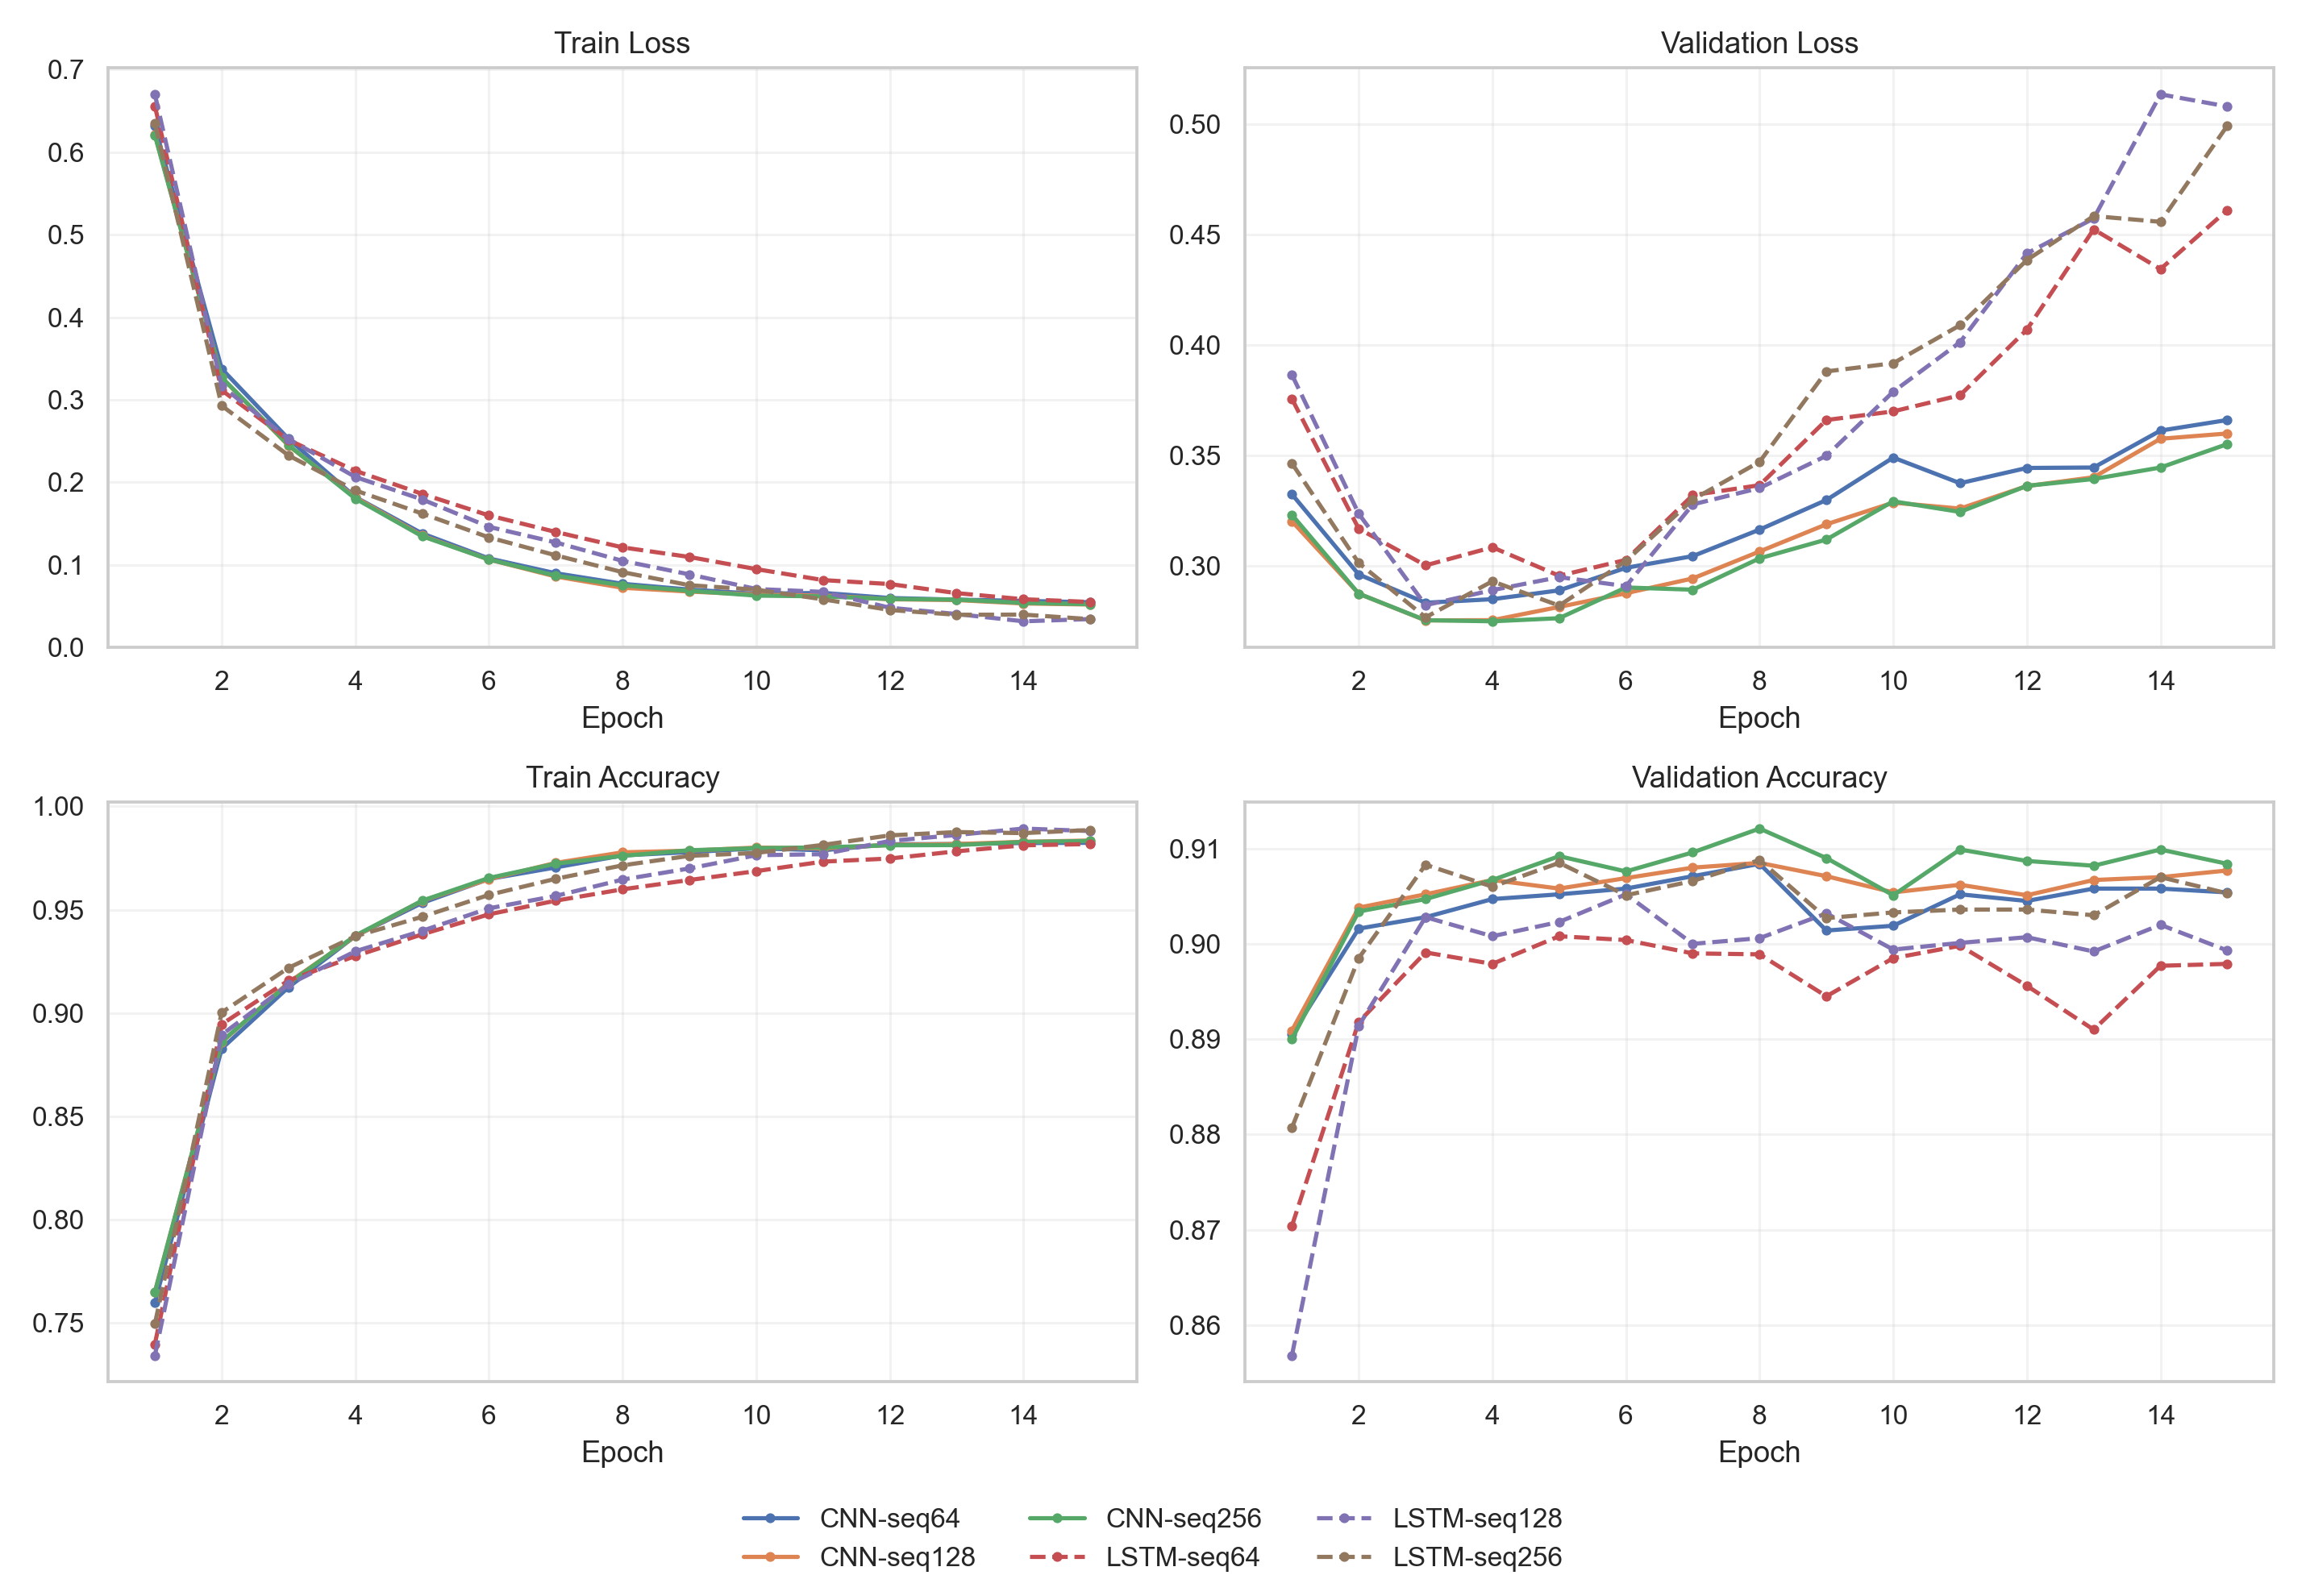
\includegraphics[width=0.95\textwidth]{../figures/generated/full_training_curves_comparison.png}
\caption{Training and validation loss/accuracy curves for all six runs. Both models show rapid early convergence and stable learning trajectories.}
\label{fig:full_training_curves_comparison}
\end{figure}

Both models show rapid convergence, with validation loss decreasing sharply in the first few epochs and then stabilizing. Both models converge to similar final validation accuracies at a similar number of epochs (e.g., around 1--2 epochs). The CNN shows a slightly more stable validation loss curve, while the LSTM shows signs of overfitting after epoch 4, where the validation loss starts to increase while training loss continues to decrease. Most notably, the LSTM at seq256 converges more rapidly as indicated by the steepest initial drop in validation loss, which may explain its superior performance at this sequence length. However, all models converge to similar final validation accuracies.
\subsection{Summary}

The LSTM model achieves the best overall result at the longest sequence length (seq256), with a test macro-F1 of 90.74\%, outperforming the CNN's best macro-F1 of 90.72\% at seq64. The LSTM benefits more from longer sequences, while the CNN performs best at shorter sequences. Both models show stable tuning and learning trajectories, with the Business class being the most challenging to classify.
